\documentclass[
]{jss}

%% recommended packages
\usepackage{orcidlink,thumbpdf,lmodern}

\usepackage[utf8]{inputenc}

\author{
Timothy Christensen~\orcidlink{0000-0002-4639-5015}\\New York University
and\\
University College London \And Xiaohong
Chen~\orcidlink{0000-0003-1125-675X}\\Yale University \And Jeffrey S.
Racine~\orcidlink{0000-0002-5680-3705}\\McMaster University
}
\title{Estimation and Confidence Bands for Nonparametric Instrumental
Variables Models: ~The \proglang{R} Package \pkg{npiv}}

\Plainauthor{Timothy Christensen, Xiaohong Chen, Jeffrey S. Racine}
\Plaintitle{Estimation and Confidence Bands for Nonparametric
Instrumental Variables Models: The R Package \pkg{npiv}}
\Shorttitle{\pkg{npiv}: Estimation and Confidence Bands for
Nonparametric IV Models}


\Abstract{
Nonparametric instrumental variables (NPIV) methods are widely used in
economics and have been adopted in other fields including causal
inference in biostatistics and machine learning. This article discusses
the \proglang{R} package \pkg{npiv}, which implements novel, fully
data-driven NPIV estimation and inference methods proposed in
\citet{CCK}. The main methods implemented in this package are (i)
data-driven, rate-optimal choices of sieve dimension for sieve NPIV
estimators and (ii) data-driven uniform confidence bands for the
structural function and its derivatives. Additional functionality allows
for constructing (non-data driven) uniform confidence bands based on the
methods proposed in \citet{CCQE}. All methods subsume standard
nonparametric regression as a special case.
}

\Keywords{nonparametric instrumental variables, nonparametric
regression, minimax rate-adaptive estimation, adaptive uniform
confidence bands, \proglang{R}}
\Plainkeywords{keywords, not capitalized, Java}

%% publication information
%% \Volume{50}
%% \Issue{9}
%% \Month{June}
%% \Year{2012}
%% \Submitdate{}
%% \Acceptdate{2012-06-04}

\Address{
    Timothy Christensen\\
    New York University and\\
University College London\\
    Department of Economics\\
  E-mail: \email{timothy.christensen@nyu.edu}\\
  URL: \url{https://tmchristensen.com}\\~\\
      Xiaohong Chen\\
    Yale University\\
    Cowles Foundation for Research in Economics and\\
Department of Economics\\
  E-mail: \email{xiaohong.chen@yale.edu}\\
  URL: \url{https://economics.yale.edu/people/faculty/xiaohong-chen}\\~\\
      Jeffrey S. Racine\\
    McMaster University\\
    Department of Economics and\\
Graduate Program in Statistics\\
  E-mail: \email{racinej@mcmaster.ca}\\
  URL: \url{https://socialsciences.mcmaster.ca/people/racinej}\\~\\
  }


% tightlist command for lists without linebreak
\providecommand{\tightlist}{%
  \setlength{\itemsep}{0pt}\setlength{\parskip}{0pt}}




\usepackage{amsmath} \usepackage{amsfonts}

\begin{document}



\hypertarget{introduction}{%
\section{Introduction}\label{introduction}}

Nonparametric instrumental variables (NPIV) methods are
well-established, widely used, and have been adopted by practitioners in
a range of empirical fields. While there is a relatively long tradition
of their use in demand estimation in economics
\citep{BCK, BHP, BerryHaile2014}, NPIV methods have recently been
adopted in non-economic areas including causal inference in
biostatistics \citep{WangZhiTT2018} as well as reinforcement learning
\citep{grettonRL2021} and, more generally, causal machine learning
\citep{causalML}. The basic premise underlying NPIV is that we are
interested in estimating a nonparametric \emph{structural function}
\(h_0\) linking a scalar outcome variable \(Y\) and a vector of
regressors \(X\) through the relation \begin{equation}\label{eq:npiv}
 Y = h_0(X) + u,
\end{equation} where \(u\) is a disturbance term. Unlike a standard
nonparametric regression model, the function \(h_0\) is not necessarily
the conditional mean of \(Y\) given \(X\) but rather has a particular
\emph{structural} or \emph{causal} interpretation. Equivalently, \(X\)
is \emph{endogenous} in the sense that \(\E[u|X]\) is not necessarily
zero. NPIV methods allow for the estimation of \(h_0\) using a vector of
\emph{instrumental variables} \(W\) for which
\(\E[u|W] = 0\).\footnote{To simplify exposition, we shall omit the
  ``almost surely'' qualifier when specifying conditional moment
  restrictions.} For instance, in a demand estimation context the
variable \(Y\) denotes the quantity demanded, \(X\) denotes the price,
and \(W\) is a ``cost-shifter'' that causes variation in the marginal
cost of production. Derivatives of \(h_0\) may also be of interest as
they have important ``structural'' interpretations as elasticities or
other marginal effects.

This article discusses the \proglang{R} package \pkg{npiv}, which
implements novel, fully data-driven NPIV estimation and inference
methods for \(h_0\) and derivatives of \(h_0\) proposed in \citet{CCK}.
The methods are developed in the context of sieve NPIV estimators, which
are implemented in a very simple and straightforward manner using
two-stage least-squares (TSLS) \citep{AC, NP}.

The main methods implemented in this package are (i) a data-driven
choice of sieve dimension for sieve NPIV estimators and (ii) data-driven
uniform confidence bands (UCBs) for the structural function and its
derivatives. As shown in \citet{CCK}, the single data-driven choice of
sieve dimension is adaptive to the optimal (i.e., minimax) sup-norm rate
for estimating both \(h_0\) and derivatives of \(h_0\). Moreover, the
data-driven \emph{uniform} confidence bands contain the entire true
structural function and its derivatives with desired asymptotic coverage
probability and contract at the optimal rate (up to log terms).
Additional functionality allows for constructing (non-data driven) UCBs
based on the methods proposed in \citet{CCQE} as well as
\emph{pointwise} confidence intervals for \(h_0(x)\) or its derivatives
at a point \(x\) based on the method of \citet{ChenPouzo}. All methods
subsume standard nonparametric regression as a special case.

The remainder of this article is organized as follows.
\protect\hyperlink{method}{Section 2} reviews sieve NPIV estimators and
describes the data-driven methods from \citet{CCK} and the UCB
constructions from \citet{CCQE}. \protect\hyperlink{desc}{Section 3}
gives a description of the main functionality of the package \pkg{npiv}
and describes its implementation. \protect\hyperlink{engel}{Section 4}
then illustrates the methods in the context of Engel curve estimation
based on household consumption data.

\hypertarget{method}{%
\section{Method}\label{method}}

\hypertarget{sieve-npiv-estimators}{%
\subsection{Sieve NPIV estimators}\label{sieve-npiv-estimators}}

The exposition in this section closely follows \citet{CCK}. We being by
briefly describing sieve NPIV estimators. Consider approximating an
unknown structural function \(h_0\) using a linear combination of \(J\)
basis functions, denoted \(\psi_{J1},\ldots,\psi_{JJ}\):
\begin{equation}\label{eq:h0_approx}
 h_0(x) \approx \sum_{j=1}^J c_{Jj} \psi_{Jj}(x) = (\psi^J(x))'c_J\,,
\end{equation} where
\(\psi^J(x) = (\psi_{J1}(x),\ldots,\psi_{JJ}(x))^\top\) is a vector of
basis functions and \(c_J = (c_{J1},\ldots,c_{JJ})^\top\) is a vector of
coefficients. Combining (\ref{eq:npiv}) and (\ref{eq:h0_approx}), we
obtain \[
 Y = (\psi^J(X))^\top c_J + \mathrm{bias}_J + u\,,
\] where \(\mathrm{bias}_J = h_0(X) - (\psi^J(X))^\top c_J\) and
\(u = Y - h_0(X)\) satisfies \(\E[u|W] = 0\). Provided
\(\mathrm{bias}_J\) is ``small'' relative to \(U\), we have an
approximate linear IV model where \(\psi^J(X)\) is a \(J\times 1\)
vector of ``endogenous variables'' and \(c_J\) is a vector of unknown
``parameters''. One can then estimate \(c_J\) using TSLS using
\(K \geq J\) transformations
\(b^K(W)= (b_{K1}(W),\ldots,b_{KK}(W))^\top\) of \(W\) as instruments.

Given data \((X_i,Y_i,W_i)_{i=1}^n\), the TSLS estimator of \(c_J\) is
simply \[
 \hat c_J = \left(\mathbf \Psi_J^\top \mathbf P_K^{\phantom \top} \mathbf \Psi_J^{\phantom \top} \right)^{-} \mathbf \Psi_J^\top \mathbf P_K^{\phantom \top} \mathbf Y \,,
\] where \(\mathbf \Psi_J = (\psi^J({X_1}),\ldots,\psi^J({X_n}))^\top\)
and \(\mathbf B_K = (b^K({W_1}),\ldots,b^K({W_n}))^\top\) are
\(n \times J\) and \(n \times K\) matrices,
\(\mathbf P_K = \mathbf B_K^{\phantom \prime} (\mathbf B_K^\top \mathbf B_K^{\phantom \top})^{-} \mathbf B_K^\top\)
is the projection matrix onto the instrument space,\footnote{We let
  \(A^-\) denote the generalized (or Moore--Penrose) inverse of a matrix
  \(A\).} and \(\mathbf Y = (Y_1,\ldots,Y_n)^\top\) is an \(n \times 1\)
vector. Sieve NPIV estimators of \(h_0\) and its derivative
\(\partial^a h_0\) are given by \[
 \hat h_J(x) = (\psi^J(x))^\top \hat c_J \,,~~~~\partial^a \hat h_J(x) =(\partial^a \psi^J(x))^\top \hat c_J \,,
\] where
\(\partial^a \psi^J(x) = (\partial^a \psi_{J1}(x),\ldots,\partial^a \psi_{JJ}(x))^\top\)
and \[
 \partial^a h(x) = \frac{\partial^{|a|} h(x)}{\partial^{a_1} x_1 \ldots \partial^{a_d} x_d} \,,
\] for \(a = (a_1,\ldots,a_d) \in (\mathbb{N}_0)^d\) with
\(|a| = a_1 + \ldots + a_d\).

The estimator \(\hat h_J\) collapses to a standard nonparametric series
regression estimator \[
 \hat h_J(x) = \psi^J(x)^\top(\mathbf \Psi_J^\top\mathbf \Psi_J^{\phantom \top})^- \mathbf \Psi_J^\top \mathbf Y
\] in the special case in which \(W = X\), \(K = J\), and
\((b_{K1},\ldots,b_{KK}) = (\psi_{J1},\ldots,\psi_{JJ})\). The
data-driven methods for choosing \(J\) and for constructing UCBs for
\(h_0\) and its derivatives therefore carry over to standard
nonparametric regression models as a special case.

In practice, a researcher must choose bases
\(\psi_{J1},\ldots,\psi_{JJ}\) and \(b_{K1},\ldots,b_{KK}\) and the
tuning parameters \(J\) and \(K\). Previously, \citet{CCQE} showed that
B-spline and certain wavelet bases lead to estimators of \(h_0\) and its
derivatives that converge at the minimax sup-norm rate under an
appropriate choice of \(J\) and \(K\). These bases also lead to
estimators that converge at the optimal rate in the special case of
nonparametric regression \citep{BCCK, CC15Reg}, again under an
appropriate choice of sieve dimension. We therefore use B-spline bases
in what follows as these are easier to compute than wavelet bases. We
generally construct bases for multivariate \(X\) or \(W\) by taking
tensor products of univariate bases.\footnote{The exception is when
  \(X\) is multivariate and we wish to impose an additively separable
  structure on \(h_0\).}

The key tuning parameter to be chosen when implementing sieve NPIV
estimators is the dimension \(J\) of the basis used to approximate
\(h_0\). Note that the bias of sieve NPIV estimators is decreasing in
\(J\) because \(h_0\) is approximated over a richer set of basis
functions. On the other hand, the variance (or sampling uncertainty) is
increasing in \(J\) because there are more coefficients to estimate.
Choices of \(J\) that appropriately balance bias against sampling
uncertainty will lead to estimators that converge at optimal rates.
However, bias and sampling uncertainty depend on certain model
regularities, such as the smoothness of \(h_0\) and the strength of the
instruments, which are unknown. It is therefore very important to have
data-driven methods for choosing tuning parameters that can \emph{adapt}
to these unknown model regularities.

\hypertarget{data-driven-choice-of-sieve-dimension}{%
\subsection{Data-driven choice of sieve
dimension}\label{data-driven-choice-of-sieve-dimension}}

\citet{CCK} introduce a data-driven choice of \(J\) that leads to
estimators of both \(h_0\) and its derivatives that converge at the
optimal sup-norm rate. The choice of \(K\) is pinned down by \(J\) in
their procedure, so we write \(K(J)\), \(b^{K(J)}(W)\),
\(\mathbf B_{K(J)}\) and \(\mathbf P_{K(J)}\) in what follows.

Before describing the procedure of \citet{CCK} we first introduce some
notation. Let \(\mathcal T\) denote the set of feasible values of \(J\).
This set depends on the choice of basis. For instance, if \(X\) is
\(d\)-dimensional and \(\psi_{J1},\ldots,\psi_{JJ}\) is the tensor
product of \(r\)-th degree univariate B-spline bases, then
\(\mathcal T = \{(2^l + r)^d : l \in \mathbb N_0 \}\). In particular,
with a univariate cubic B-spline basis we have
\(\mathcal T = \{4,5,7, 11, ...\}\). Let
\(J^+ = \min\{j \in \mathcal T : j > J\}\) be the smallest sieve
dimension in \(\mathcal T\) exceeding \(J\).

Let
\(\mathbf M_J = (\mathbf \Psi_J^\top \mathbf P_{K(J)}^{\phantom \top} \mathbf \Psi_J^{\phantom \top} )^{-} \mathbf \Psi_J^\top \mathbf P_{K(J)}^{\phantom \top}\).
For \(J,J_2 \in \mathcal T\) with \(J_2 > J\), define \[
D_{J}(x)-D_{J_2}(x) = (\psi^J(x))^\top \mathbf M_J \hat{\mathbf  u}_J - (\psi^{J_2}(x))^\top \mathbf M_{J_2} \hat{\mathbf u}_{J_2} \,.
\] The contrast \(D_{J}(x)-D_{J_2}(x)\) compares the estimates of
\(\hat h_J(x) - h_0(x)\) and \(\hat h_{J_2}(x) - h_0(x)\). Its variance
is estimated by \[
 \hat \sigma_{J,J_2}^2(x) := \hat \sigma_{J}^2(x) + \hat \sigma_{J_2}^2(x) - 2 \tilde \sigma_{J,J_2}(x),
\] where \[
 \hat \sigma_{J}^2(x) =  (\psi^J(x))^\top \mathbf M_J^{\phantom \top} \widehat{\mathbf U}_{J,J}^{\phantom \top} \mathbf M_J^\top \psi^J(x)
\] and \[
 \tilde \sigma_{J,J_2}(x)  = (\psi^J(x))^\top \mathbf M_J^{\phantom \top} \widehat{\mathbf U}_{J,J_2}^{\phantom \top} \mathbf M_{J_2}^\top \psi^{J_2}(x),
\] with \(\widehat{\mathbf U}_{J,J_2}\) an \(n\times n\) diagonal matrix
whose \(i\)th diagonal entry is \(\hat u_{i,J} \hat u_{i,J_2}\). A
bootstrap version of the contrast is given by \[
D_{J}^*(x)-D_{J_2}^*(x) = (\psi^J(x))^\top\mathbf M_J^{\phantom \top}  \hat{\mathbf u}_J^* - (\psi^{J_2}(x))^\top \mathbf M_{J_2}^{\phantom \top} \hat{\mathbf u}_{J_2}^*,
\] with
\(\hat{\mathbf u}_J^* = (\hat u_{1,J}\varpi_1,\ldots,\hat u_{n,J}\varpi_n)^\top\)
denoting a multiplier bootstrap version of \(\hat{\mathbf u}_J\), where
\((\varpi_i)_{i=1}^n\) are IID \(N(0,1)\) draws independent of the data.

Finally, let \(\hat s_J\) be the smallest singular value of
\((\mathbf B_{K(J)}^\top\mathbf B_{K(J)}^{\phantom \top})^{-1/2} (\mathbf B_{K(J)}^\top \mathbf \Psi_J^{\phantom \top}) (\mathbf \Psi_J^\top \mathbf \Psi_J^{\phantom \top})^{-1/2}\).

The data-driven procedure from \citet{CCK} for choosing \(J\) in NPIV
models is summarized in the following three steps:

\begin{enumerate}
\item Compute 
\begin{equation}\label{eq:index_set}
 \hat{\mathcal J}  = \left\{ J \in \mathcal T : 0.1 ( \log \hat J_{\max})^2 \leq J \leq \hat J_{\max}\right\}
\end{equation}
where
\begin{equation} \label{eq:J_hat_max}
 \hat{J}_{\max} = \min \bigg \{ J \in \mathcal T :   J \sqrt{\log J}  \hat{s}_J^{-1}     \leq 10 \sqrt{n}  <  J^{+} \sqrt{\log J^{+}}   \hat{s}_{J^{+}}^{-1}  \bigg \} \,.
\end{equation}
\item Let $\hat \alpha = \min\{ 0.5 , (\log(\hat{J}_{\max})/\hat{J}_{\max})^{1/2}\}$.  For each independent draw of $(\varpi_i)_{i=1}^n$, compute
\begin{equation}\label{eq:sup-stat}
 \sup_{\{ (x,J,J_2) \in \mathcal{X} \times \hat{\mathcal J} \times \hat{\mathcal J} : J_2 > J \}} \left| \frac{D_{J}^*(x)-D_{J_2}^*(x)}{\hat \sigma_{J,J_2}(x)} \right|.
\end{equation}
Let $\theta^*_{1-\hat \alpha}$ denote the $(1- \hat \alpha )$ quantile of the sup statistic (\ref{eq:sup-stat}) across a large number  of independent draws of $(\varpi_i)_{i=1}^n$.
\item Let $\hat J_n = \max\{J \in \hat{\mathcal J} : J < \hat J_{\max}\}$ and
\begin{equation}\label{eq:J_lepski}
 \hat{J} = \min \left \{ J \in \hat{\mathcal J} : \sup_{(x, J_2) \in \mathcal{X} \times \hat{\mathcal{J}} : J_2 > J } \left| \frac{D_{J}(x)-D_{J_2}(x)}{\hat \sigma_{J,J_2}(x)} \right| \leq 1.1 \theta^*_{1 - \hat \alpha} \right \} \,.
\end{equation}
The data-driven choice of sieve dimension is
\begin{equation} \label{eq:J-choice}
 \tilde{J} = \min\{\hat{J},\hat J_n\}\,.
\end{equation}
\end{enumerate}

\citet{CCK} show that the single data-driven choice \(\tilde J\) leads
to estimators \(\hat h_{\tilde J}\) and \(\partial^a \hat h_{\tilde J}\)
of \(h_0\) and \(\partial^a h_0\) that converge at the optimal sup-norm
rate in NPIV models. They also show that these adaptivity guarantees
carry over to standard nonparametric regression models with \(W = X\),
\(K = J\), and
\((b_{K1},\ldots,b_{KK}) = (\psi_{J1},\ldots,\psi_{JJ})\). In that case,
the procedure is implemented largely as above, but with the following
slight modifications:

\begin{enumerate}
\item[$1.^{\prime}$] Compute
\begin{equation} \label{eq:J_hat_max_regression}
 \hat{J}_{\max} = \min \bigg \{ J \in \mathcal T :   J \sqrt{\log J} \upsilon_n \leq 10 \sqrt n <  J^{+} \sqrt{\log J^{+}} \upsilon_n  \bigg \}
\end{equation}
with $\upsilon_n = \max\{1, (0.1 \log n)^4\}$, then compute $\hat{\mathcal J}$ as in (\ref{eq:index_set}) with this choice of $\hat J_{\max}$.
\item[$2.^{\prime}$] As above.
\item[$3.^{\prime}$] Take $\tilde J = \hat J$ for $\hat J$ defined in (\ref{eq:J_lepski}).
\end{enumerate}

\hypertarget{data-driven-uniform-confidence-bands}{%
\subsection{Data-driven uniform confidence
bands}\label{data-driven-uniform-confidence-bands}}

We now describe the method for constructing UCBs for \(h_0\) and its
derivatives proposed in \citet{CCK}. The approach builds on the
data-driven choice of \(J\) introduced in the previous subsection.
Recall \(\hat{\mathcal J}\) and \(\tilde J\) from above. Let
\(\hat A = \log \log \tilde J\) and \[
 \hat{\mathcal J}_{-} =
 \begin{cases}
 \{J \in \hat{\mathcal J} : J < \hat J_n\} & \mbox{~if $\tilde J = \hat J$}, \\
 \hat{\mathcal J} & \mbox{~if $\tilde J = \hat J_n$}.
 \end{cases}
\]

UCBs for the structural function \(h_0\) in NPIV models are constructed
in the following steps:

\begin{enumerate}
\item[4.] For each independent draw of $(\varpi_i)_{i=1}^n$, compute
\begin{equation} \label{eq:z_star-UCB}
 \sup_{(x,J) \in \mathcal{X} \times \hat{\mathcal J}_{-}} \left| \frac{D_J^*(x)}{\hat \sigma_J(x)} \right|.
\end{equation}
Let $z_{1-\alpha}^*$ denote the $(1-\alpha )$ quantile of the sup statistic (\ref{eq:z_star-UCB}) across a large number of independent draws of $(\varpi_i)_{i=1}^n$.
\item[5.] Construct the 100$(1-\alpha)$\% UCB
\begin{equation} \label{band}
 C_n(x) = \bigg[ \hat{h}_{\tilde{J}}(x) - \left( z_{1-\alpha}^* + \hat A \theta^*_{1-\hat \alpha}  \right ) \hat \sigma_{\tilde J}(x) , ~  \hat{h}_{\tilde{J}}(x) + \left( z_{1-\alpha}^* + \hat A \theta^*_{1-\hat \alpha}  \right) \hat \sigma_{\tilde J}(x) \bigg] \,.
\end{equation}
\end{enumerate}

UCBs for derivatives \(\partial^a h_0\) of the structural function in
NPIV models are constructed analogously:

\begin{enumerate}
\item[$4.^{\prime}$] For each independent draw of $(\varpi_i)_{i=1}^n$, compute
\begin{equation} \label{eq:z_star-UCB-derivative}
 \sup_{(x,J) \in \mathcal{X} \times \hat{\mathcal J}_{-}} \left| \frac{D_J^{a*}(x)}{\hat \sigma_J^a(x)} \right|.
\end{equation}
Let $z_{1-\alpha}^{a*}$ denote the $(1-\alpha )$ quantile of sup statistic (\ref{eq:z_star-UCB-derivative}) across a large number of independent draws of $(\varpi_i)_{i=1}^n$.
\item[$5.^{\prime}$] Construct the 100$(1-\alpha)$\% UCB
\begin{equation} \label{band-derivative}
 C_n^a(x) = \bigg[ \partial^a \hat{h}_{\tilde{J}}(x) - \left(\! z_{1-\alpha}^{a*} + \hat A \theta^*_{1-\hat \alpha} \! \right) \hat \sigma_{\tilde J}^a(x) ,~ \partial^a \hat{h}_{\tilde{J}}(x) + \left( \!z_{1-\alpha}^{a*} + \hat A \theta^*_{1-\hat \alpha} \! \right ) \hat \sigma_{\tilde J}^a(x) \bigg] .
\end{equation}
\end{enumerate}

The above UCB constructions apply equally to standard nonparametric
regression models in the special case in which \(W = X\), \(K = J\), and
\((b_{K1},\ldots,b_{KK}) = (\psi_{J1},\ldots,\psi_{JJ})\).

\citet{CCK} establish uniform asymptotic coverage guarantees for these
UCBs for both NPIV and standard nonparametric regression models. They
also show that the UCBs contract at the optimal sup-norm rate (up to
logarithmic factors).

\hypertarget{uniform-confidence-bands-based-on-undersmoothing}{%
\subsection{Uniform confidence bands based on
undersmoothing}\label{uniform-confidence-bands-based-on-undersmoothing}}

An alternative UCB construction based on a deterministic (i.e.,
non-data-driven) choice of sieve dimension is proposed by \citet{CCQE}
for NPIV models. The construction also applies to standard nonparametric
regression in the special case in which \(W = X\), \(K = J\), and
\((b_{K1},\ldots,b_{KK}) = (\psi_{J1},\ldots,\psi_{JJ})\). The
theoretical justification for this approach is based on
\emph{undersmoothing}. That is, the sieve dimension \(J\) should be
larger than what would be optimal for estimation, so that bias is of
smaller order than sampling uncertainty.

We now briefly summarize their procedure using the notation introduced
above. UCBs for \(h_0\) and \(\partial^a h_0\) are constructed as
follows:

\begin{enumerate}
\item For each independent draw of $(\varpi_i)_{i=1}^n$, compute
\begin{equation} \label{eq:z_star-J-UCB}
 \sup_{x\in \mathcal{X}} \left| \frac{D_J^*(x)}{\hat \sigma_J(x)} \right|~\mbox{for $h_0$, or}~~~~\sup_{x \in \mathcal{X}} \left| \frac{D_J^{a*}(x)}{\hat \sigma_J^a(x)} \right|~\mbox{for $\partial^a h_0$}.
\end{equation}
Let $z_{1-\alpha,J}^*$ and $z_{1-\alpha,J}^{a*}$ denote the $(1-\alpha )$ quantile of
these sup statistics across a large number of independent draws of $(\varpi_i)_{i=1}^n$.
\item Construct the $100(1-\alpha)\%$ UCBs
\[
 C_{n,J}(x) = \bigg[ \hat{h}_{J}(x) -  z_{1-\alpha,J}^* \hat \sigma_{J}(x) , ~  \hat{h}_{J}(x) + z_{1-\alpha,J}^* \hat \sigma_{J}(x) \bigg] ~\mbox{for $h_0$},
\]
or
\[
 C_{n,J}^a(x) = \bigg[ \partial^a \hat{h}_{J}(x) - z_{1-\alpha,J}^{a*} \hat \sigma_{J}^a(x) ,~ \partial^a \hat{h}_{J}(x) +  z_{1-\alpha,J}^{a*} \hat \sigma_{J}^a(x) \bigg] ~\mbox{for $\partial^a h_0$}.
\]
\end{enumerate}

\hypertarget{pw}{%
\subsection{Pointwise confidence intervals based on
undersmoothing}\label{pw}}

Finally, we note that it may sometimes be of interest to construct
confidence intervals (CIs) for \(h_0(x)\) or \(\partial^a h_0(x)\) at a
certain point \(x\). To this end, one may use the following
constructions for \(100(1-\alpha)\%\) CIs: \[
 \bigg[ \hat{h}_{J}(x) -  z_{1-\alpha/2} \hat \sigma_{J}(x) , ~  \hat{h}_{J}(x) + z_{1-\alpha/2} \hat \sigma_{J}(x) \bigg] ~\mbox{for $h_0(x)$},
\] or \[
 \bigg[ \partial^a \hat{h}_{J}(x) - z_{1-\alpha/2} \hat \sigma_{J}^a(x) ,~ \partial^a \hat{h}_{J}(x) +  z_{1-\alpha/2} \hat \sigma_{J}^a(x) \bigg] ~\mbox{for $\partial^a h_0(x)$},
\] where \(z_{1-\alpha/2}\) is the \(1-\alpha/2\) quantile of the
\(N(0,1)\) distribution; see \citet{ChenPouzo} and Appendix D of
\citet{CCQE} for a formal justification for these constructions. These
CIs can be (and sometimes are) plotted alongside estimates of \(h_0\) or
\(\partial^a h_0\), but it should be understood that they are only valid
\emph{pointwise}. That is, they will generally be too narrow to contain
the entire function \(h_0\) or \(\partial^a h_0\) with desired
asymptotic coverage probability. By contrast, the above UCB
constructions will contain the true structural function or its
derivatives with desired asymptotic coverage probability.

\hypertarget{desc}{%
\section{Package description}\label{desc}}

The contributed \proglang{R} package \pkg{npiv} is used to estimate and
construct UCBs for a nonparametric structural function \(h_0\) and its
derivatives \(\partial^a h_0\) in both NPIV and standard nonparametric
regression models. In this section, we describe the main functionality
of this package. The current version of the package can be downloaded
from GitHub:

\begin{verbatim}
library(devtools); install_github('JeffreyRacine/npiv')
\end{verbatim}

\hypertarget{use-in-npiv-models}{%
\subsection{Use in NPIV models}\label{use-in-npiv-models}}

The main function is \texttt{npiv()}, which can be called with the
following syntax:

\begin{verbatim}
npiv(formula, data, newdata=NULL, basis=c("tensor","additive","glp"),
     J.x.degree=3, J.x.segments=NULL, 
     K.w.degree=4, K.w.segments=NULL, K.w.smooth=2, ...)
\end{verbatim}

The required arguments include

\begin{itemize}
\item
  \texttt{formula}: a symbolic formula specifying the model to be
  estimated. The syntax is the same as the package \pkg{ivreg}
  \citep{IVREG}. For example,
  \texttt{y\ \textasciitilde{}\ x1\ +\ x2\ \textbar{}\ x1\ +\ z1\ +\ z2}
  where \texttt{y} is the dependent variable, \texttt{x1} is an
  exogenous regressor, \texttt{x2} is an endogenous regressor, and
  \texttt{z1} and \texttt{z2} are instrumental variables.
\item
  \texttt{data}: an optional data frame containing the variables in the
  model.
\item
  \texttt{newdata}: optional data frame collecting the values of
  \texttt{x} variables at which to evaluate the estimator (e.g.~for
  plotting). Will evaluate at sample data points if \texttt{NULL}.
\item
  \texttt{basis}: type of basis to use if \texttt{x} variables are
  multivariate. Default is \texttt{tensor} for a tensor-product basis.
  Can also use \texttt{additive} for an additively-separable structural
  function or \texttt{glp} for generalized B-spline polynomial bases
  (for further details, see documentation for the package \pkg{crs}
  \citep{CRS}).
\item
  \texttt{J.x.degree}: degree of the B-spline used to approximate the
  structural function. Default is 3 (cubic spline).
\item
  \texttt{J.x.segments}: number of segments (interior knots plus 1) for
  the B-spline used to approximate the structural function. Note that
  integers for both \texttt{J.x.segments} and \texttt{K.w.segments} must
  be passed to estimate the model with a deterministic \(J\) (and \(K\))
  and return undersmoothed UCBs. Te default is \texttt{NULL}, in which
  case both \texttt{J.x.segments} and \texttt{K.w.segements} are
  data-determined using the procedure described above and data-driven
  UCBs are returned.
\item
  \texttt{K.w.degree}: degree of the B-spline used to approximate the
  nonparametric first stage. Default is 4 (quartic spline).
\item
  \texttt{K.w.segments}: number of segments (interior knots plus 1) for
  the B-spline used to approximate the structural function. Note that
  integers for both \texttt{J.x.segments} and \texttt{K.w.segments} must
  be passed to estimate the model with a deterministic \(J\) (and \(K\))
  and return undersmoothed UCBs. The default is \texttt{NULL}, in which
  case both \texttt{J.x.segments} and \texttt{K.w.segements} are
  data-determined using the procedure described above and data-driven
  UCBs are returned.
\item
  \texttt{K.w.smooth}: a non-negative integer. The basis for the
  nonparametric first-stage uses \texttt{2\^{}\{K.w.smooth\}} more
  B-spline segments for each instrument than the basis approximating the
  structural function. Default is 2. Setting \texttt{K.w.smooth=0} uses
  the same number of segments for \texttt{x} and \texttt{w}.
\end{itemize}

The output of the function \texttt{npiv()} is a `\texttt{npiv}' object.
The \texttt{summary()} method prints a brief summary of the estimated
model. The \texttt{npiv} object includes the following components:

\begin{itemize}
\item
  \texttt{h}: the estimated structural function evaluated at the sample
  data (or evaluation data, if provided).
\item
  \texttt{h.upper}: the upper UCB for the structural function evaluated
  at the sample data (or evaluation data, if provided).
\item
  \texttt{h.lower}: the lower UCB for the structural function evaluated
  at the sample data (or evaluation data, if provided).
\item
  \texttt{deriv}: estimated derivative of the structural function
  evaluated at the sample data (or evaluation data, if provided).
\item
  \texttt{h.upper.deriv}: the upper UCB for the derivative of the
  structural function evaluated at the sample data (or evaluation data,
  if provided).
\item
  \texttt{h.lower.deriv}: the lower UCB for the derivative of the
  structural function evaluated at the sample data (or evaluation data,
  if provided).
\item
  \texttt{asy.se}: pre-asymptotic standard errors for the estimator of
  the structural function evaluated at the sample data (or evaluation
  data, if provided). These may be used to construct (pointwise)
  confidence intervals for \(h_0(x)\) based on undersmoothing when a
  deterministic sieve dimension is used.
\item
  \texttt{deriv.asy.se}: pre-asymptotic standard errors for the
  estimator of the derivative of the structural function evaluated at
  the sample data (or evaluation data, if provided). These may be used
  to construct (pointwise) confidence intervals for
  \(\partial^a h_0(x)\) based on undersmoothing when a deterministic
  sieve dimension is used.
\item
  \texttt{K.w.segments}: value of \texttt{K.w.segments} used (will be
  data-determined if not provided).
\item
  \texttt{J.x.segments}: value of \texttt{J.x.segments} used (will be
  data-determined if not provided).
\item
  \texttt{beta}: vector of estimated spline coefficients \(\hat c_J\).
\end{itemize}

\hypertarget{use-in-standard-nonparametric-regression-models}{%
\subsection{Use in standard nonparametric regression
models}\label{use-in-standard-nonparametric-regression-models}}

The command \texttt{npiv()} may also be used for data-driven choice of
sieve dimension and UCB construction in standard nonparametric
regression models. In this case, \texttt{formula} should pass the same
explanatory variables as instrumental variables (and in the same order).
Calling

\begin{verbatim}
npiv(y ~ x1 + x2 | x1 + x2)
\end{verbatim}

will perform nonparametric regression of \texttt{y} on \texttt{x1} and
\texttt{x2}, with a data-driven choice of sieve dimension. Note that
this choice of sieve dimension will be rate-optimal for estimation of
\(h_0\) and its derivatives under sup-norm loss. This choice may differ
from the choice of sieve dimension selected by other methods that target
mean-square error (i.e., \(L^2\)-norm loss), such as cross validation,
because the optimal choices of sieve dimension for estimation under
sup-norm and \(L^2\)-norm losses diverge at different rates. As before,
data-driven UCBs for the conditional mean function and its derivative
will also be computed by default using the procedure of \citet{CCK}.

Estimators based on a deterministic choice of sieve dimension and
undersmoothed UCBs can be computed by passing \texttt{J.x.segments}.
Both \texttt{K.w.segments} and \texttt{K.w.smooth} are redundant and do
not need to be specified. Undersmoothed UCBs are constructed using the
procedure of \citet{CCQE}; see also \citet{BCCK}. Standard errors
\texttt{asy.se} and \texttt{deriv.asy.se} may also be used to construct
(pointwise) confidence intervals for \(h_0(x)\) and
\(\partial^a h_0(x)\) based on undersmoothing, using the method
described in \protect\hyperlink{pw}{Section 2.5}.

\newpage

\hypertarget{additional-options}{%
\subsection{Additional options}\label{additional-options}}

By default, \texttt{npiv} will perform estimation of the structural
function \(h_0\) and construct 95\% UCBs for \(h_0\) and
\(\frac{d h_0}{dx}\) if \(x\) is scalar or \[
 \frac{\partial h_0(x_1,\ldots,x_d)}{\partial x_1}
\] if \(x\) is multivariate. The following optional arguments can be
used to modify the UCB constructions:

\begin{itemize}
\item
  \texttt{alpha}: nominal size of the uniform confidence bands. Default
  is 0.05 for 95\% uniform confidence bands.
\item
  \texttt{deriv.index}: integer indicating for which regressor to
  compute the derivative. Default is \texttt{1} for differentiation with
  respect to \(x_1\).
\item
  \texttt{deriv.order}: integer indicating the order of derivative to be
  computed. Default is \texttt{1}.
\item
  \texttt{ucb.h}: whether to compute a uniform confidence band for the
  structural function. Default is \texttt{TRUE.}
\item
  \texttt{ucb.deriv}: whether to compute a uniform confidence band for
  the derivative of the structural function. Default is \texttt{TRUE}.
\end{itemize}

Run time can be improved by passing \texttt{ucb.h\ =\ FALSE} or
\texttt{ucb.deriv\ =\ FALSE} when a UCB for \(h_0\) or its derivative
are not required.

\hypertarget{engel}{%
\section{Engel curve estimation}\label{engel}}

We now illustrate the usage of \texttt{npiv} with an empirical
application to nonparametric Engel curve estimation \citep{BCK}. Engel
curves explain how consumers' expenditure shares on different categories
of goods and services vary as a function of total household expenditure.
Understanding consumers' consumption and substitution patterns across
expenditure categories is important for conducting policy analysis and
for modeling demand. Engel curve estimation is therefore the subject of
a large amount of empirical work in economics. There is also a long
tradition of estimating Engel curves via ``flexible'' (i.e.,
nonparametric or semi-parametric) methods which recognize correctly that
consumers' expenditure shares vary nonlinearly with total
expenditure.\footnote{Interestingly, the original empirical exercise
  performed by Engel over 150 years ago used precursors of nonparametric
  statistical methods \citep{CM}.}

We wish to estimate the Engel curve \(h_0\) for a household's
expenditure share on a particular category, say food. The model is \[
 Y_i = h_0(X_i) + u_i
\] where \(Y_i\) is expenditure share for household \(i\) on food and
\(X_i\) is log total household expenditure. The ``structural''
interpretation of the model is that the household would spend the
fraction \(h_0(x)\) of its total expenditure on food if log total
expenditure was exogenously specified as \(x\). As is well known (see,
e.g., \citet{BBL}), total household expenditure is endogenous: \[
 \E[Y_i | X_i] \neq h_0(X_i),
\] which follows from the fact that the household's consumption
preferences determines its expenditure across categories and therefore
its total expenditure. To deal with this endogeneity, we shall follow
\citet{BBL}, \citet{BCK}, and several other works and use log gross
earnings of the household head (\(W_i\), hereafter log wages) as an
instrument for log total expenditure.

We use data from the 1995 British Family Expenditure Survey as in
\citet{BCK}. The data consist of 1655 married or cohabitating couples
with the head of household employed and aged between 20 and 55 and with
zero, one, or two children. The data are available as part of \pkg{npiv}
in the data frame \texttt{Engel95}.

\begin{CodeChunk}
\begin{CodeInput}
R> data("Engel95", package = "npiv")
R> head(Engel95)
\end{CodeInput}
\begin{CodeOutput}
       food   catering    alcohol       fuel      motor      fares    leisure
1 0.1494936 0.10459980 0.00000000 0.07554642 0.19400656 0.03446044 0.16236387
2 0.3646063 0.03262203 0.01532990 0.09762080 0.19944200 0.03679176 0.13520971
3 0.2104212 0.06524783 0.07918546 0.03367232 0.25255781 0.01002152 0.17813644
4 0.0786906 0.11526845 0.07013521 0.05841701 0.00000000 0.24973512 0.02726338
5 0.2824394 0.05508218 0.07504724 0.15707207 0.21778214 0.00000000 0.03753635
6 0.1663630 0.15928116 0.17427441 0.02050462 0.09070033 0.00000000 0.14901404
    logexp logwages nkids
1 4.877561 5.533113     0
2 5.094241 5.371289     0
3 5.781675 6.001043     0
4 5.756296 5.860758     0
5 5.279863 6.569341     0
6 5.821521 5.879247     0
\end{CodeOutput}
\end{CodeChunk}

The first seven columns of \texttt{Engel95} list household budget shares
across different expenditure categories. The variables \texttt{logexp}
and \texttt{logwages} are log total household expenditure and log wages
The final variable \texttt{nkids} indicates whether the household has
zero children (if \texttt{nkids\ =\ 0}; 628 households in total), or 1-2
two children (if \texttt{nkids\ =\ 1}; 1027 households in total).

We first estimate the Engel curve for food. To try to ensure a
relatively homogeneous set of households, we focus on the subset of
households with 1-2 children.

\begin{CodeChunk}
\begin{CodeInput}
R> Engel.kids <- subset(Engel95, nkids == 1)
R> attach(Engel.kids)
\end{CodeInput}
\end{CodeChunk}

To use a data-driven choice of sieve dimension and construct data-driven
UCBs for \(h_0\) and its derivative, we first call \texttt{npiv()}
without specifying the sieve dimensions. We also pass a grid of points
spanning \([4.75, 6.25]\) for plotting the estimator and confidence
bands:

\begin{CodeChunk}
\begin{CodeInput}
R> newdata <- data.frame(logexp = seq(4.75, 6.25, length.out = 1000))
R> fm.food.dd <- npiv(food ~ logexp | logwages, newdata = newdata)
R> summary(fm.food.dd)
\end{CodeInput}
\begin{CodeOutput}
Call:
npiv.formula(formula = food ~ logexp | logwages, newdata = newdata)

Nonparametric IV Model:

IV Regression Data: 1027 training points, and 1000 evaluation points, in 1 endogenous variable(s)

B-spline degree for instruments:             4
B-spline segments for instruments:           4

B-spline degree for endogenous predictors:   3
B-spline segments for endogenous predictors: 1

Estimation time: 1.8 seconds
\end{CodeOutput}
\end{CodeChunk}

As \(X\) and \(W\) are both scalar and we use the default cubic B-spline
basis for \(X\) and quartic B-spline basis for \(W\), the data-driven
choice of sieve dimension are therefore \(J = 4\) and \(K = 8\) (the sum
of segments and degree for each basis). The run time represents the
total time to perform data-driven choice of sieve dimension and to
construct the data-driven UCBs for \(h_0\) and its derivative.

To compare data-driven and undersmoothed UCBs, we estimate \(h_0\) and
its derivative again, this time using a deterministic choice of \(J\)
and \(K\) by passing both \texttt{J.x.segments} and
\texttt{K.w.segments}. As the justification for the UCBs is
undersmoothing, we must choose a \(J\) and \(K\) larger than the optimal
value so that bias is of smaller order than sampling uncertainty. We
choose to estimate with \texttt{J.x.segments\ =\ 2} and
\texttt{K.w.segments\ =\ 5}, which corresponds to \(J = 5\) and
\(K = 9\).

\begin{CodeChunk}
\begin{CodeInput}
R> fm.food.det <- npiv(food ~ logexp | logwages, newdata = newdata, 
+                     J.x.segments = 2, K.w.segments = 5)
\end{CodeInput}
\end{CodeChunk}

The estimated Engel curves for food are plotted below, together with
their UCBs (using \texttt{h.upper} and \texttt{h.lower}). Both the
data-driven and undersmoothed estimates are downward-sloping. This seems
reasonable from an economic standpoint: food is a necessary good, and so
it should decrease as a proportion of total household expenditure as
total household expenditure increases. Note, however, that the
data-driven estimate looks close to linear whereas the undersmoothed
estimate is more wiggly. The undersmoothed UCBs are also wider over much
of the support of total expenditure because they use a sub-optimally
large choice of sieve dimension and are therefore less ``efficient''
than the data-driven bands. We also plot 95\% pointwise confidence
intervals (PCIs) based on undersmoothing (using \texttt{asy.se} and a
\(N(0,1)\) critical value). As expected, these are narrower than the
UCBs based on undersmoothing as they are only required to contain the
true function at each point, rather than over the entirety of its
support. So while PCIs can be used for drawing inference about the value
of the function at a given point, they cannot be used for inferring the
true shape of the function.

\begin{figure}
\centering
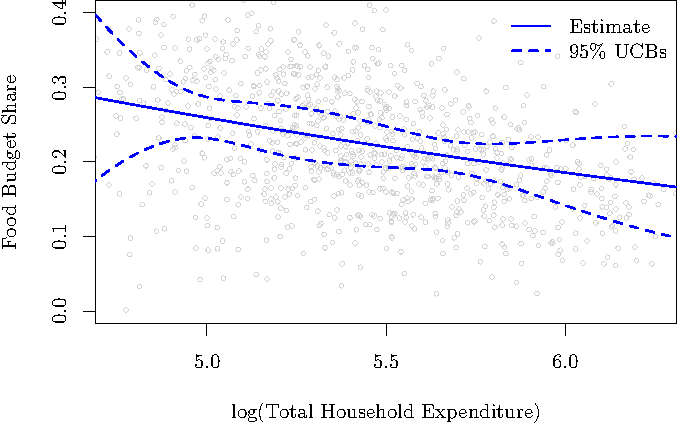
\includegraphics{npiv_files/figure-latex/food-dd-1.pdf}
\caption{Engel Curve for Food: Data-driven Estimates and UCBs}
\end{figure}

\begin{figure}
\centering
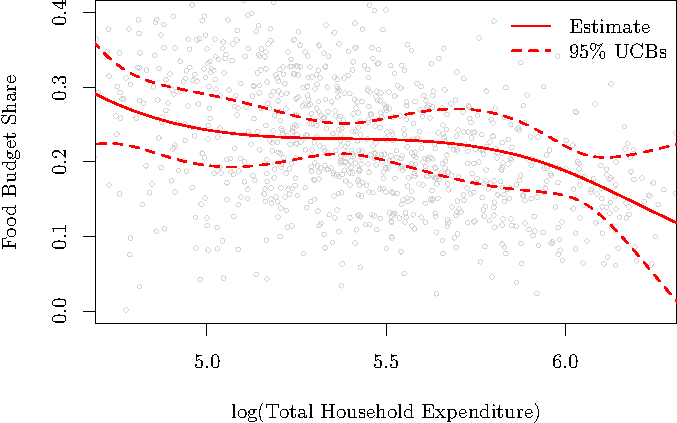
\includegraphics{npiv_files/figure-latex/food-det-1.pdf}
\caption{Engel Curve for Food: Estimates, UCBs, and PCIs based on
Undersmoothing}
\end{figure}

These differences between the data-driven and undersmoothed methods are
also apparent when we compare the estimated derivatives of the Engel
curves and their corresponding UCBs (using \texttt{h.lower.deriv} and
\texttt{h.upper.deriv}). The zero function lies significantly above the
data-driven UCBs over a sub-interval of total expenditure, indicating
that the true Engel curve is significantly downwards-sloping over this
region. Therefore, one may conclude from the data-driven UCBs that the
Engel curve for food differs significantly from a constant.

Conversely, the UCBs based on undersmoothing are wider, and appear to
contain the zero function over the full range of total expenditure.
Hence, one cannot reject a flat Engel curve using the UCBs based on
undersmoothing. We also report PCIs for the derivative based on
undersmoothing (using on \texttt{deriv.asy.se} and \(N(0,1)\) critical
values). These are useful for testing hypotheses about the derivative at
a \emph{given} point, but that is a different problem from testing
whether the derivative is significantly different from zero at
\emph{any} point over its support.

\begin{figure}
\centering
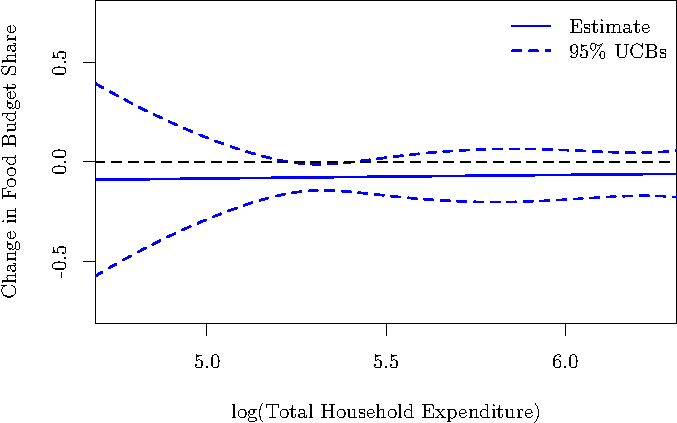
\includegraphics{npiv_files/figure-latex/food-dd-deriv-1.pdf}
\caption{Engel Curve Derivative for Food: Data-driven Estimates and
UCBs}
\end{figure}

\begin{figure}
\centering
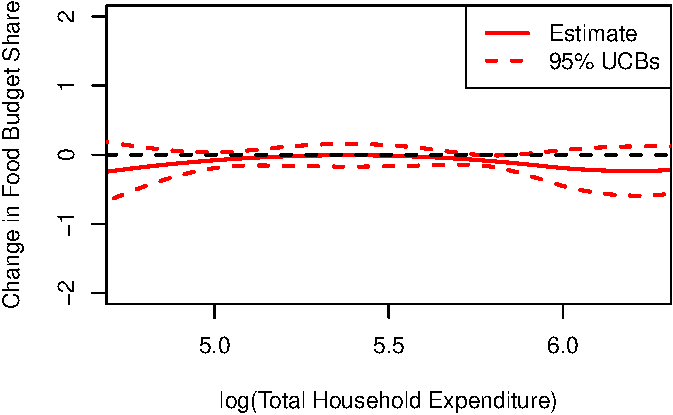
\includegraphics{npiv_files/figure-latex/food-det-deriv-1.pdf}
\caption{Engel Curve Derivative for Food: Estimates, UCBs, and PCIs
based on Undersmoothing}
\end{figure}

We repeat the above exercise, this time estimating an Engel curve for
household budget share on fuel:

\begin{CodeChunk}
\begin{CodeInput}
R> fm.fuel.dd <- npiv(fuel ~ logexp | logwages, newdata = newdata)
R> summary(fm.fuel.dd)
\end{CodeInput}
\begin{CodeOutput}
Call:
npiv.formula(formula = fuel ~ logexp | logwages, newdata = newdata)

Nonparametric IV Model:

IV Regression Data: 1027 training points, and 1000 evaluation points, in 1 endogenous variable(s)

B-spline degree for instruments:             4
B-spline segments for instruments:           4

B-spline degree for endogenous predictors:   3
B-spline segments for endogenous predictors: 1

Estimation time: 1.8 seconds
\end{CodeOutput}
\end{CodeChunk}

We see from the estimated Engel curve and its derivative that budget
shares on fuel decrease significantly at low total expenditure levels
and then flatten out completely at moderate to high total expenditure
levels. As there is much less variation in households' fuel expenditure
than their food expenditure, these curves are estimated with greater
precision and the UCBs are correspondingly much narrower.

\begin{figure}
\centering
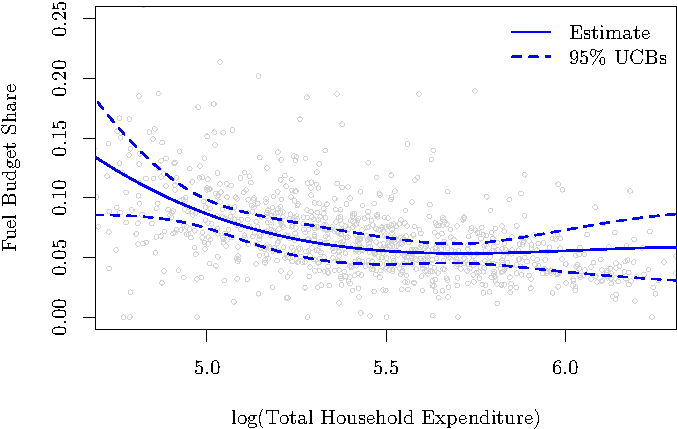
\includegraphics{npiv_files/figure-latex/fuel-dd-1.pdf}
\caption{Engel Curve for Fuel: Data-driven Estimates and UCBs}
\end{figure}

\begin{figure}
\centering
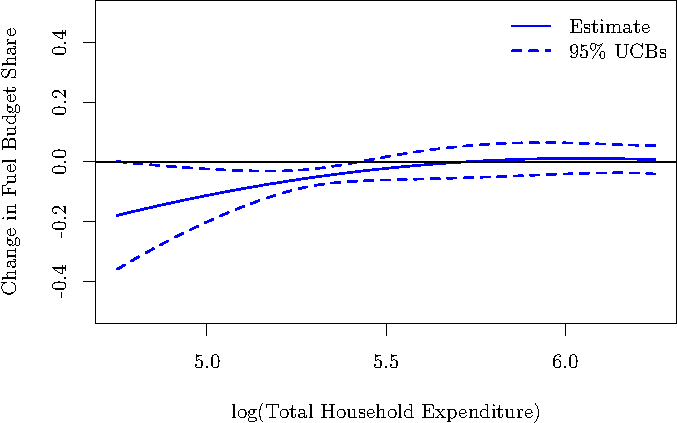
\includegraphics{npiv_files/figure-latex/fuel-dd-deriv-1.pdf}
\caption{Engel Curve Derivative for Fuel: Data-driven Estimates and
UCBs}
\end{figure}

\bibliography{npiv.bib}



\end{document}
